\chapter{Basic Concepts}
\label{cap:Basic}

Most real networks, like social, biological, and technological networks present many non-trivial topological features, with patterns of connection between their elements that are neither purely regular nor purely random. These features include the scale-free, the small-world and community structure properties. In this work we are interested in investigating whereas these properties occur in Twitter multilayer ego networks. Besides, we are also interested in analyzing similarities and dissimilarities among layers of the multilayer ego networks considered. Thus, in this chapter we present the concepts and the related measures we use to answer our main research questions.

At the outset, section \ref{sec:graphs} is the definition of graphs, with their main characteristics. Graphs are mathematical models used in this work for the representation of multilayer ego networks. In section \ref{sec:graph_properties}, we list some of the main properties of graphs and how they are used in the network analysis process. In section \ref{sec:net_models} are described some models that represent phenomena found in the real networks and that help to understand the structures of the networks. In sections \ref{sec:important_vertices} and \ref{sec:vertex_edges_overlap} we investigate the similarity between the layers of the same multilayer ego network. Finishing this chapter, the section \ref{sec:communities} is devoted to describing concepts that involve one of the major structures exhibited by OSNs, the communities, approaching detection algorithms and evaluation metrics of these structures in graphs.


%%%%%%%%%%%%%%%%%%%%%%%%%%%%%%%%%%%%%%%%%%%%%%%%%%%%%%%%
%%%%%%%%%%%%%%%%%%%%%%%%%%%%%%%%%%%%%%%%%%%%%%%%%%%%%%%%

\section{Graphs}
\label{sec:graphs}

Graphs can be understood as mathematical models used to represent relationships between objects of a given set and is usually used to model network structures. The notation of a graph $\mathcal{G}$ can be developed as a set of vertices $\mathcal{V}$, representing the objects of a network, and a set of edges $\mathcal{E}$ that connect the vertices and represent the relationships between the pairs of objects. Mathematically speaking, the graph $\mathcal{G}$ is expressed by Eq. \ref{eq:graph}:

\begin{equation} 
    \label{eq:graph}
    \mathcal{G}=(\mathcal{V},\mathcal{E}),
\end{equation}

where $\mathcal{V}$ is the set of vertices $\mathcal{V}=\{v_1, v_2, . . . , v_n\}$, with $v_i, 1 \leq i \leq n$ being a single vertex; and $\mathcal{E}$ is the set of edges $\mathcal{E}=\{e_1, e_2, . . . , e_m\}$, with $e_i, 1 \leq i \leq m$, being a single edge. 

The edges are formed by a tuple $e(v_1,v_2), v_1, v_2 \in \mathcal{V}$ which indicates a connection between the vertices $v_1$ and $v_2$. Since the edges connect two vertices, we have $\mathcal{E} \subseteq \mathcal{V} \times \mathcal{V}$. The number of vertices $|\mathcal{V}|$ indicates the {\em order} of the graph and the number of edges $|\mathcal{E}|$ indicates the {\em size} of the graph.

The vertices of a graph can also be called nodes or actors depending on the context and subject in which they are being used. In this dissertation we will use the term {\em vertices} to refer to the set of objects modeled in graphs. In OSNs the set of vertices represents the entities, or generally called users, that is, people, companies, computer systems, etc., that create and manage profiles in the virtual environment made available by OSNs; and the set of edges represent the interactions that take place between these users. For example, the graph shown in Fig. \ref{fig:ex_graph_undir} models the friendship relationship between seven users of a fictional OSN. Each user is represented by a vertex, drawn as a circle. There is an edge between two users only if they maintain a friendly relationship in OSN. A line connecting two vertices is the representation of an edge.

\begin{figure}[htb]
	\centering
	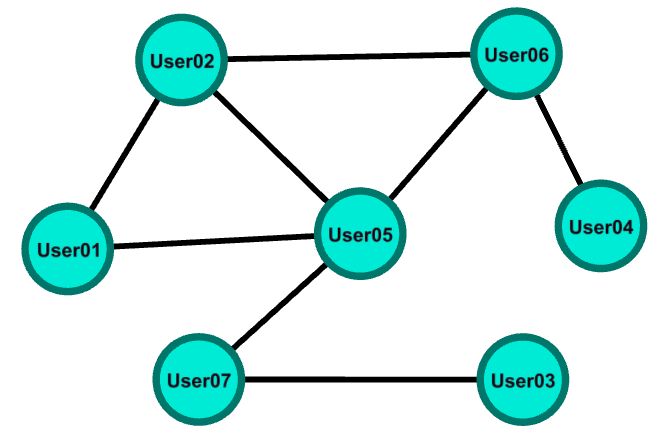
\includegraphics[width=0.8\textwidth]{fig/intro/ex_graph_undir.png}
	\caption{Example of a graph representing the friendship relationship between users of an OSN.}
	\label{fig:ex_graph_undir}
\end{figure}

The friendship interaction represented in Fig. \ref{fig:ex_graph_undir} indicates that each pair of users are friends when there is an edge linking them, or they are not friends if there is no edge linking them. This means that in the example cited, user {\em User01} is friend of user {\em User02} and vice versa. The graph that models this type of relationship is called an undirected graph, and the edges are formed by unordered pairs of vertices that model a bidirectional relationship. In an undirected graph $\mathcal{G} = (\mathcal{V}, \mathcal{E})$, the edge $e(a,b)$, $a, b \in \mathcal{V}$ is the same edge $e(b,a)$, $a, b \in \mathcal{V}$.

Graphs can also be used to model unidirectional relationships between vertices pairs. Sending a message from user $a$ to user $b$ on an OSN, for example, is a type of one-way relationship. In cases like these, the constructed graph should show the direction of the relationships. These graphs are called directed graphs, digraphs, and an edge, which can also be called an arc, is formed by an ordered pair of vertices, called initial vertex (tail) and terminal vertex (head). In this dissertation we will use only the term {\em edges} to refer to the connection between two vertices of a graph. The representation of the edges is made by arrows that start from an initial vertex and arrive at a terminal vertex (head). In a directed graph $\mathcal{G} = (\mathcal{V}, \mathcal{E})$, the edge $e(a,b)$, $a, b \in \mathcal{V}$ is different from the edge $e(b,a)$, $ a, b \in \mathcal{V}$.

\begin{figure}[htb]
	\centering
	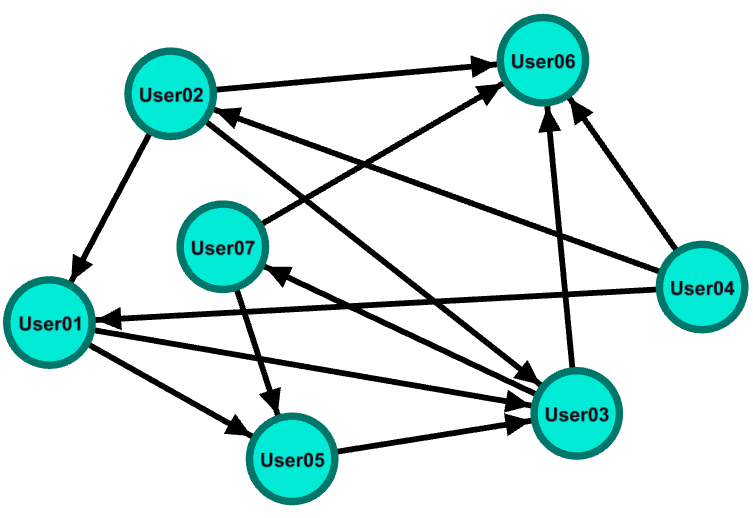
\includegraphics[width=0.8\textwidth]{fig/intro/ex_graph_dir.png}
	\caption{Example of a directed graph representing relationships arising from message sending interactions between users of an OSN.}
	\label{fig:ex_graph_dir}
\end{figure}

The Fig. \ref{fig:ex_graph_dir} illustrates the example of a directed graph that models interactions associated with sending messages between users. In this type of interaction, there is the definition of a sender, user that promotes the interaction, that is, the initial vertex of the edge, and a recipient, who receives the message and is the terminal vertex of the edge. Therefore, it is necessary for the edge to indicate the flow of information to represent the interaction in a correct way, different from the example with the friendship interaction, in which the edge only needs to indicate whether there is interaction (friendship) or not.

Two vertices are {\em adjacent} if they are connected by an edge. Adjacency can also be referenced as {\em neighborhood}. The adjacent vertices (neighbors) of a vertices $a$ form the neighborhood of $a$. In the case of a directed graph, the neighborhood is divided into: (i) successors - the vertex $b$ is successor of $a$ if there is an edge that starts from $a$ and arrives at $b$; and (ii) predecessors - the vertex $a$ is the predecessor of $b$ if there is an edge that goes from $a$ to $b$. The notation used for the neighborhood of a vertex $a$ in a graph $\mathcal{G}$ is represented by Eq. \ref{eq:neighborhood}:


\begin{equation} 
    \label{eq:neighborhood}
    N_\mathcal{G}(a)
\end{equation}

and is called the open neighborhood of $a$ when $a$ is not enclosed, or closed neighborhood of $a$ when $a$ is enclosed. The vertices neighborhood can be used to represent graphs in computer algorithms and are also used to identify properties of graphs.

Graphs can also have subgraphs. A subgraph of $\mathcal{G}$ is a graph whose set of vertices is a subset of the set of vertices of $\mathcal{G}$ and the set of edges is a subset of the set of edges of $\mathcal{G}$. Formally we have that for any graph $\mathcal{G}=(\mathcal{V},\mathcal{E})$ a graph  $\mathcal{G'}=(\mathcal{V'},\mathcal{E'})$ is a subgraph of  $\mathcal{G}=(\mathcal{V},\mathcal{E})$ if it holds the following properties:

\begin{itemize}
    \item $\mathcal{V'} \subseteq \mathcal{V}$,
    \item $\mathcal{E'} \subseteq (\mathcal{V'} \times \mathcal{V'}) \cap \mathcal{E}$.
\end{itemize}

One can traverse a graph starting from one point to another through paths formed by vertices and edges. A distance $k$ between two vertices $a$ and $b$, is defined as $p(a,b)_k$, and is an alternating sequence of vertices and edges that starts at $a$ and ends in $b$, according to Eq. \ref{eq:path_lenght_k}:

\begin{equation}
    \label{eq:path_lenght_k}
    p(a,b)_k = v_0,e_1,v_1,e_2,v2,...,e_k,v_k
\end{equation}

such that, (i) $a=v_0$ and $b=v_k$; (ii) there is at least one edge; (iii) for $1 \leq i \leq k$ the edge $e_i$ connect the vertices $v_{i-1}$ and $v_i$.


If the graph is undirected, the vertices that are bounded by the $e_i$ edge are $v_i$ and $v_{i+1}$, otherwise, $e_i$ is an edge that starts from $v_i$ and ends in $v_{i+1}$. The length of the walk is defined by the number of edges that it has, or, in weighted graphs, by the weight of the edges of the path, which also corresponds to the distance of the path. A walk that does not pass twice through the same vertex is called {\em path}. A walk that begins and ends at the same vertex and there are no repeated edges is called {\em circuit}, and a circuit that does not have repeated vertices is called {\em cycle}.

For a directed graph $\mathcal{G}$, we say that $C_{a,b}$ is a shortest path between vertices $a$ and $b$ if there is no other path that starts at $a$ and ends at $b$ (or vice versa in undirected graphs) of lesser length that $C_{a,b}$, that is, $C_{a,b}= min(p(a,b))$. If there is no path from $a$ to $b$, we can say that the distance from $a$ to $b$ is infinite.

%%%%%%%%%%%%%%%%%%%%%%%%%%%%%%%%%%%%%%%%%%%%%%%%%%%%%%%%
%%%%%%%%%%%%%%%%%%%%%%%%%%%%%%%%%%%%%%%%%%%%%%%%%%%%%%%%


\section{Graph Properties}
\label{sec:graph_properties}
The analysis of a network passes through the understanding of its structure, which can be made from the graphs teory, according to the properties exhibited by them. The properties analyzed allow us to evaluate the graph for aspects related to its vertices and connections, for example, to determine which are the central vertices, shortest paths between the vertices, degree of connection of the vertices, etc. In OSNs, the analysis of these properties is essential for the correct understanding of the dynamics of formation of communities, such as the identification of cohesive groups, their central vertices, vertices of connection with other groups, estimation of the flow of information transmitted between vertices, etc. Here are some of the main properties of graphs:

\begin{itemize}
	\item \textbf{Order -} the order of a graph represents the number of vertices in the graph: $o(G) = |\mathcal{V}|$.
        	
    \item \textbf{Size:} the size of a graph is indicated by the number of vertices plus the number of links between them: $s(G) = |\mathcal{V}| + |\mathcal{E}|$.
        
    \item \textbf{Average Degree -} Indicates the number of connections that, on average, each vertex of the graph has. In the case of OSNs, this measure must be interpreted with caution because the degree distribution generally does not follow a normal distribution, as it was possible to observe in Fig. \ref{fig:twitter_degree_distr}, therefore, the average has no representativity. However, even so, this propertie helps in comparing different networks. The average degree is defined according to Eq. \ref{eq:avg_degree}:
    \begin{equation}
        \label{eq:avg_degree}
    	d(G) = \frac{1}{|\mathcal{V}|} \sum_{v \in \mathcal{V}}d_G(v).
    \end{equation}
        
	\item \textbf{Eccentricity -} the eccentricity of a vertex $v$ corresponds to the maximum distance between $v$ and any other vertex $u$ of the graph: $e(v) = max_{u \in \mathcal{V}}d(u,v)$.

    \item \textbf{Diameter -} The diameter of a network represents the largest distance between two vertices of the network, that is, the greatest eccentricity. This propertie is useful for evaluating the maximum distance an information would need to travel to reach two vertices in a network using only shortest paths, that is, it reveals the number of minimum connections required to connect two vertices of the network. It is calculated by observing the greatest of all shortest paths between the vertices, according Eq. \ref{eq:diameter}:
    	\begin{equation}
    	    \label{eq:diameter}
        	d = max_{v \in \mathcal{V}}e(v).
    	\end{equation}
        
    \item \textbf{Radius -} the radius of the network is equal to the shortest path between two vertices, that is, the smallest eccentricity: $r = min_{v \in \mathcal{V}}e(v)$.
            
    \item \textbf{Center -}: A vertex $v$ is in the center of the network if the radius of the network is equal to the eccentricity of the vertex $v$: $e(v) = r$.
        
    \item \textbf{Periphery -} A vertex $v$ is at the periphery, if its eccentricity is equal to the diameter of the network: $e(v) = d$.
    	
    \item \textbf{Density -} The density of a network is defined as the ratio of edges to the number of possible edges. For directed graphs the density is calculated according Eq. \ref{eq:density_directed}:
        \begin{equation}
            \label{eq:density_directed}
            D=\frac {|\mathcal{E}|}{|\mathcal{V}|(|\mathcal{V}|-1)}.
    	\end{equation}
    
    For undirected graphs, each edge must be counted twice, according Eq. \ref{eq:density_undirected}:
        \begin{equation}
            \label{eq:density_undirected}
            D=\frac {2|\mathcal{E}|}{|\mathcal{V}|(|\mathcal{V}|-1)}.
    	\end{equation}
\end{itemize}

\subsection*{Degree Centrality}
\label{subsec:degree_centr}
The degree centrality of a vertex $a$ is defined as the number of edges associated with it ($d_a$), which also corresponds to the number of adjacent vertices. A zero-degree vertex is called an isolated vertex. In unirected graphs, the sum of the degrees of all vertices is equal to twice the number of edges of the graph, according to Eq. \ref{eq:node_degree_undirected}:

\begin{equation} 
\label{eq:node_degree_undirected}
    \sum_{i}d_i = 2\left | \mathcal{E} \right |,
\end{equation}

since each edge links two vertices. In directed graphs, the degree of a vertex $a$ is decomposed into {\em indegree} ($d_a^{in}$) and {\em outdegree} ($d_a^{out}$), the which corresponds, respectively, to the number of edges that arrive at the vertex, that is, the number of edges in which the vertex $a$ is the terminal vertex, and the number of edges that start from the vertex, that is, the number of edges where $a$ is the initial vertex. Therefore, the degree of a vertex $a$ is formed by the sum of the indegree and the outdegree, as Eq: \ref{eq:node_degree_directed}:

\begin{equation} 
\label{eq:node_degree_directed}
    d_a = d_a^{in} + d_a^{out},
\end{equation}

and the sum of all indegrees is equal to the sum of all outdegrees, in accordance with Eq. \ref{eq:node_degree_directed_total}:

\begin{equation}
\label{eq:node_degree_directed_total}
    \sum_{i}d_i^{in} = \sum_{j}d_j^{out}.
\end{equation}

A special case of binding in a graph is the {\em loop}, which occurs when an edge attaches a vertex to itself. In undirected graphs, each loop adds two to the degree of the vertex that owns it, as this will be identified as initial vertex and terminal vertex for the edge of the loop. It is worth remembering that in the case of a directed graph, each loop will add one to the indegree and one to the outdegree of the vertex that owns it.

When working with graphs of the order of thousands of vertices, or even larger than this, it is important to evaluate initially the distribution of degrees of vertices. The distribution $p_d$ is the probability that a randomly selected vertex has degree $d$. In a graph with $n$ vertices, $p_d$ is defined according to Eq. \ref{eq:prob_degree}:

\begin{equation}
    \label{eq:prob_degree}
    p_d = \frac{n_d}{n},
\end{equation}

where $n_d$ is the number of vertices with degree $d$. Figure \ref{fig:twitter_degree_distr} gives the example of the probability distribution through the representation of the Twitter mentions network in April 2017\footnote{\textit{Twitter network dataset - KONECT, April 2017}. \url{http://konect.uni-koblenz.de/networks/munmun_twitterex_at}}. Each vertex of this network is a Twitter user and a directed edge indicates a direct message sent from one user to another. The degree of each vertex is given by the sum of the indegree and the outdegree. It can be observed that, in this example, most users have a very low degree, while a much smaller number of users have a high degree.

\begin{figure}[htb]
	\centering
	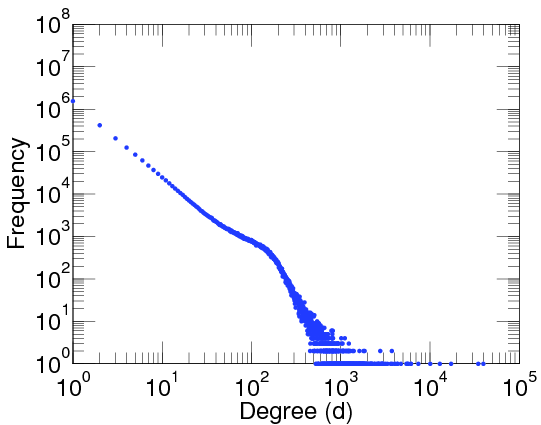
\includegraphics[width=0.8\textwidth]{fig/intro/twitter_degree_distr.png}
	\caption{Distribution of degrees from the Twitter mentions network - April 2017.}
	\label{fig:twitter_degree_distr}
\end{figure}


\subsection*{Betweenness Centrality}
\label{subsec:betweenness_centr}
The betweenness centrality evaluates the importance of the vertices and edges as to the capacity to serve as a link between the elements of the network. One of the ways of calculating the centrality of intermediation is presented in \cite{Zafarani2014}, in which the authors demonstrate that for a given vertex $v$, we compute the number of shortest paths between two other vertices that pass through vertex $v$, according to Eq. \ref{eq:spl}:

\begin{equation}
    \label{eq:spl}
    C_b(v) = \sum_{s \neq t \neq v} \frac{\sigma_{st}(v)}{\sigma_{st}},
\end{equation}
        
where $\sigma_{st}$ is the minimum number of paths from $s$ to $t$ and $\sigma_{st}(v)$ is the number of shortest paths from $s$ to $t$ that pass through $v$. The same approach can also be used to calculate the edge betweeness centrality. In the case of directed graphs, the direction of the edges must be considered.

For the case of comparison between different networks, the betweenness centrality must be normalized. This normalization is given by the ratio between the betweenness centrality and the maximum that this value can have in a network. For undirected graphs the calculation can be done according to Eq. \ref{eq:bet_centr_undirected}:
\begin{equation}
    \label{eq:bet_centr_undirected}
	C^{norm}_b(v) = \frac{C_b(v)}{\binom{n-1}{2}} = \frac{C_b(v)}{((|\mathcal{V}|-1)(|\mathcal{V}|-2))/2}.
\end{equation}

In case of directed graphs, one must take into account the direction of the edge and, therefore, the formula to be used is expressed by Eq. \ref{eq:bet_centr_directed}:
\begin{equation}
    \label{eq:bet_centr_directed}
	C^{norm}_b(v) = \frac{C_b(v)}{2\binom{|\mathcal{V}|-1}{2}} = \frac{C_b(v)}{(|\mathcal{V}|-1)(|\mathcal{V}|-2)}.
\end{equation}


\subsection*{Closeness Centrality}
\label{subsec:close_centr}
The calculation of the closeness centraloty of a vertex is formulated taking into account the average of the minimum paths of the vertex to the other vertices of the network, according to Eq. \ref{eq:close_centr}:

\begin{equation}
\label{eq:close_centr}
    C_c(v) = \frac{1}{\bar{l}_{v_i}},
\end{equation}
% 1/media = valor normalizado pois na media é computado a distancia para todos os demais vértices.

where 

\begin{equation}
    \bar{l}_{v_i} = \frac{1}{|\mathcal{V}|-1}\sum_{v_j \neq v_i}l_{j,i}
\end{equation}

is the average of the minimum paths of all the others vertices for the vertex $v_i$. In this case, the greater the centrality of proximity, the closer the vertex is to the other vertices of the network. This calculation takes into account only connected graphs.


\subsection*{Reciprocity}
\label{subsec:reciprocity}
Reciprocity is the ratio between the number of edges having a corresponding edge in reverse direction and the total number of edge in a directed graph  $G = (\mathcal{V}, \mathcal{E})$. The results are in the range [0,1].  If the reciprocity of  $G$ is equal to one, then  for each edge $(u,v)\in\mathcal{E}$ there exists an edge $(v,u)\in\mathcal{E}$. Reciprocity equals to zero if  for every edge $(u,v)\in\mathcal{E}$ there is no edge $(u, v)\in\mathcal{E}$. Formally, reciprocity  of a graph $G = (\mathcal{V}, \mathcal{E})$ can be defined as:  
\begin{equation}\label{eq:reciprocity}
  reciprocity(G)=\frac{|\{(u,v)\in\mathcal{E}: (v,u) \in \mathcal{E}\}|}{|\mathcal{E}|}.
\end{equation}

\subsection*{Clustering Coefficient}  
\label{subsec:clust_coef}
A clustering coefficient is a measure of the extent to which the vertices of a graph  tend to connect to each other, forming clusters. Watts and Strogatz \cite{Watts1998} give evidence that many real graphs present  clustering coefficient  values greater than their  equivalent random graphs (i.e., a random graph with the same number of vertices and edges). In literature there are two distinct measures of clustering coefficient most used.  The first, is known as {\em global clustering coefficient} and the second is known as {\em local clustering coefficient}. The global clustering coefficient  computes the probability  of forming triangles in the graph \cite{Newman2003}. A ``triangle'' is a set of three vertices in which each is linked to the other two by an edge. The global clustering coefficient $C_G^\Delta$ of a given graph $G$ is computed as follows:

\begin{equation}
\label{eq:globClustCoef}
    C_G^\Delta = \frac{3\times \textrm{num. of triangles}}{\textrm{num. of connected triples of vertices}},
\end{equation}

where a ``connected triple'' means a single vertex with edges running to an unordered pair of others.

Given a vertex $v$ of a directed  graph $G=(V,E)$, let $N_v$ be neighbor set of $v$, i.e, the set of vertices adjacent to $v$. The local clustering coefficient $C_v$ of $v$ is defined by Watts and Strogatz \cite{Watts1998} as the ratio of number of edges between vertices in $N_v$ to the  number of edges that could possibly exist between them:

\begin{equation}
\label{eq:locClustCoef}
    C_v = \frac{|\{(v_i,v_j): v_i,v_j \in N_v, (v_i,v_j)\in E\}|}{|N_v|(|N_v|-1)}
\end{equation}

Watts and Strogatz  derived a clustering coefficient $C_G$ for the graph $G$ by averaging the local clustering coefficient of all vertex in $G$:

\begin{equation}
\label{eq:wsClustCoef}
    C_G= \frac{1}{n}\sum_{v \in V} C_v.
\end{equation}

In this work we will adopt the Watss and Strogats clustering coefficient $C_G$ as the clustering coefficient of a graph $G$. 

\subsection*{Average Shortest Path Length - ASPL}
A path between two vertices $a$ and $b$ in a graph $G=(V,E)$, is  a sequence of edges in $E$ connecting $a$ to $b$ in $G$. The length of a path  is  the number of edges in the sequence of edges forming that path. 

Once all the graphs we consider in this work are directed graphs, we computed the  ASPL value $L$ for a graph $G$ according to  \cite{Mao2013} as we next describe. Consider a graph $G(V,E)$,  with the set of vertices $V$. Let $dist(v_1,v_2)$ denote the shortest path length between vertices $v_1$ and $v_2$,  $v_1,v_2 \in V$. Assume $dist(v_1,v_2)=0$, if $v_1 =v_2$ or if $v_2$ can not be reached from $v_1$ in $G$. Also consider that $haspath(v_1,v_2)=0$ if $v_1 = v_2$ or  if there is no path from $v_1$ to $v_2$ in $G$, and $haspath(v_1,v_2)=1$ if there is a path from $v_1$ to $v2$ in $G$. The  ASPL ($L_G$) for graph $G$ is computed as:

\begin{equation}
\label{eq:ASPL}
   L_{G} = \frac{\sum\limits_{i,j}^{|V|} dist(v_i,v_j)}{\sum\limits_{i,j}^{|V|} haspath(v_i,v_j)},
\end{equation}

%%%%%%%%%%%%%%%%%%%%%%%%%%%%%%%%%%%%%%%%%%%%%%%%%%%%%%%%
%%%%%%%%%%%%%%%%%%%%%%%%%%%%%%%%%%%%%%%%%%%%%%%%%%%%%%%%


\section{Network Models}
\label{sec:net_models}
It is not always possible to perform an analysis in a real network with a high number of elements and connections, such as the OSNs, for example, due to the difficulty in obtaining the complete data and/or the high computational cost for the manipulation of the networks graphs. This section presents two models that simulate phenomena observed in real networks and allow their reproduction in smaller synthetic graphs with the same properties existing in the original graphs: Scale-Free Graphs and Small-World Graphs.

%Random Graph is built on the assumption that the relationship between the elements happens at random. The random graph model widely used in the literature is denoted by $G(n,p)$, indicating that for a graph with a fixed number of vertices $n$, the edges appear independently, with probability $p$ \cite{Solomonoff1951,Gilbert1959}. This is one of the random graphs models widely used in the literature.

\subsection{Scale-Free Graphs}
\label{sec:scale_free}
According to Barabasi et al. \cite{Barabasi509}, a scale-free graph is a graph with a few vertices with a large number of edges and numerous vertices with a small number of edges. The authors explain that this feature  was found to be a consequence of two mechanisms found in real graphs: (i) graphs expand continuously by the addition of new vertices, and (ii) new vertices attach preferentially to vertices that are already well connected. In general, this scale-free  graph follows a power-law distribution vertices degrees. The power function of a scale-free network is defined as follows:
\begin{equation}\label{eq:1}
P(k) \sim k ^{-\gamma},
\end{equation}
where $P(k)$ is the distribution of the number of vertices with $k$ degrees (connected edges) divided by the total number of vertices, according to the different $k$ values. When k is approaching to $\infty$, $P(k)$ is close to $k^{-\gamma}$. From Eq. \ref{eq:1} , $\gamma$ can be isolated, according to the following equation:

\begin{equation}\label{eq:2}
\gamma \sim \frac{\ln P(k)}{\ln k},
\end{equation}
when $\gamma <0$, $P(k)$ follows a normal distribution, when $0 < \gamma < 2$, $P(k)$ is a variant distribution of the power function that has a heavy-tailed shape. If $2 < \gamma <3$, $p(k)$ is a scale-free distribution \cite{PARK201632}.


%%%%%%%%%%%%%%%%%%%%%%%%%%%%%%%%%%%%%%%%%%%%%%%%%%%%%%%%
%%%%%%%%%%%%%%%%%%%%%%%%%%%%%%%%%%%%%%%%%%%%%%%%%%%%%%%%


\subsection{Small-World Graphs} 
\label{sec:small_worlds}
Watts and Strogatz \cite{Watts1998}, observed that many real technological, biological, social, and information graphs fall into the broad class of ‘small-world’ graphs, an intermediary  ground between regular and random graphs. Small-world graphs  have high local clustering of elements, like  regular graphs, but also short path lengths between elements, like random graphs \cite{Humphries2010}. Humphries and Gurney \cite{Humphries2010}  defined a  measure of ‘small-world-ness’, named $S$, based on the trade off between high local clustering and short path length. A  graph is  deemed a ‘small-world’ if $S>1$.
 
A graph $G $ with $n$ vertices and $m$ edges is a small-world graph  if it has a similar path length but greater clustering of vertices than an equivalent Erd\"{o}s-R\'{e}nyi (E$-$R) random graph $G_{E-R}$  with the same $m$ and $n$ \cite{bollobas01}. Let $L_G$ and $L_{E-R}$ be the average shortest path length (ASPL) over all vertex pairs of $G$ and of its equivalent $G_{E-R}$, respectively. Also, let $C_G$ and $C_{E-R}$ be the clustering coefficient of $G$ and $G_{E-R}$, respectively. Humphries and Gurney defined the $S$ measure by relating the ASPL and the clustering coefficient of both graph, according to the following equation:

\begin{equation}\label{eq:S}
    S=\frac{\Gamma_G}{\Lambda_G},
\end{equation}

where

\begin{equation}\label{eq:3}
    \Gamma_G= \frac{C_G}{C_{E-R}},
\end{equation} 

and 
\begin{equation} \label{eq:4}
    \Lambda_G= \frac{L_G}{L_{E-R}}.
\end{equation}


%%%%%%%%%%%%%%%%%%%%%%%%%%%%%%%%%%%%%%%%%%%%%%%%%%%%%%%%
%%%%%%%%%%%%%%%%%%%%%%%%%%%%%%%%%%%%%%%%%%%%%%%%%%%%%%%%
\section{Important Vertices}
\label{sec:important_vertices}
Another aspect evaluated in this work is related to the similarity when the function performed by the vertices in each layer. For this we will evaluate the centrality of the degrees and the centrality of proximity of the vertices in each layer and then investigate the similarity of these measures between the layers.

The number of edges associated to a given vertex indicates how influential this vertex is in the graph, with the ability to directly reach the other vertices. This information can be acquired by analyzing the distribution of degrees of the vertices in the network. The structural position of a given vertex reveals how important this vertex can be in the information dissemination process, with the central vertices serving as fast access bridges so that there is communication between vertices that are at the end of the graph, in addition to being able to reach all other vertices at a lower cost. Therefore, the centrality of proximity of the vertices will also be treated in this work.

\subsection*{Rank-Biased Overlap}
\label{subsec:rbo_results}
We are also interested in finding out if users with higher indegree and closeness centrality are repeated in the tops of the ranks of different layers. For this, we need a measure that gives greater value to the coincidences at the top of the rankings and that can handle the ties that take place in the two ranks. Because they are different size rankings, since the layers are of different sizes, and are made up of different elements, as proven in the Chapter \ref{cap:ExpSetup}, the measures usually used in the literature such as Kendall's Tau and Spearman's rank correlation coefficient are not suitable for the calculation of these rankings.

To analyze the rankings between layer pairs we use the Extended Rank-Biased Overlap (Extended RBO) \cite{Webber2010}, which is a measure that meets all our restrictions. The operation of the Extended RBO is based on the biased performance in the proportional overlap through a convergent series of weights according to the considered proportion of the ranking. Thus, the infinite tail of a ranking does not dominate the head. Therefore, the similarity between rankings is given from the prefix evaluation to set upper and lower bounds on the score that the full evaluation could achieve. A parameter $p$ controls the size of the prefix to be considered. Extended RBO is in the range [0,1] where 0 indicates total difference and 1 indicates equality between rankings.


%%%%%%%%%%%%%%%%%%%%%%%%%%%%%%%%%%%%%%%%%%%%%%%%%%%%%%%%
%%%%%%%%%%%%%%%%%%%%%%%%%%%%%%%%%%%%%%%%%%%%%%%%%%%%%%%%


\section{Vertex and Edge Overlap Across Layers}
\label{sec:vertex_edges_overlap}

In this article we also investigate how similar two graphs (layers) of the multilayer ego network of an ego $e$ are. In practical terms, this corresponds to investigate  the similarity between the vertex set and the similarity between the edge set of two graphs. Usually, the Jaccard similarity is used to compare two sets, but as shown in Section \ref{sec:net_structure}, there are great discrepancies on the number of vertices and on the number of edges between  pairs of graphs corresponding to distinct interactions of an ego in Twitter. Thus, we opt to use the same {\em overlap} measure used in \cite{Omodei2015} to assess  the similarity of two sets $S_1$ and $S_2$:
\begin{equation}\label{eq:overlap}
O(S_1, S_2)= \frac{|S_1\cap S_2|}{min(|S_1|, |S_2|)}.
\end{equation}


%%%%%%%%%%%%%%%%%%%%%%%%%%%%%%%%%%%%%%%%%%%%%%%%%%%%%%%%
%%%%%%%%%%%%%%%%%%%%%%%%%%%%%%%%%%%%%%%%%%%%%%%%%%%%%%%%


\section{Communities in Graphs}
\label{sec:communities}

Contrary to what is found in random graphs, where vertices have roughly the same number of edges and negligible probability of having elements with different degrees of the average, some networks, such as OSNs, for example, exhibit community structures. These structures represent dense regions where some vertices concentrate a greater number of edges \cite{FORTUNATO201075, Zhou2015b}. The particular study of the communities contributes to the understanding of the networks that have it.

\begin{figure}[htb]
	\centering
	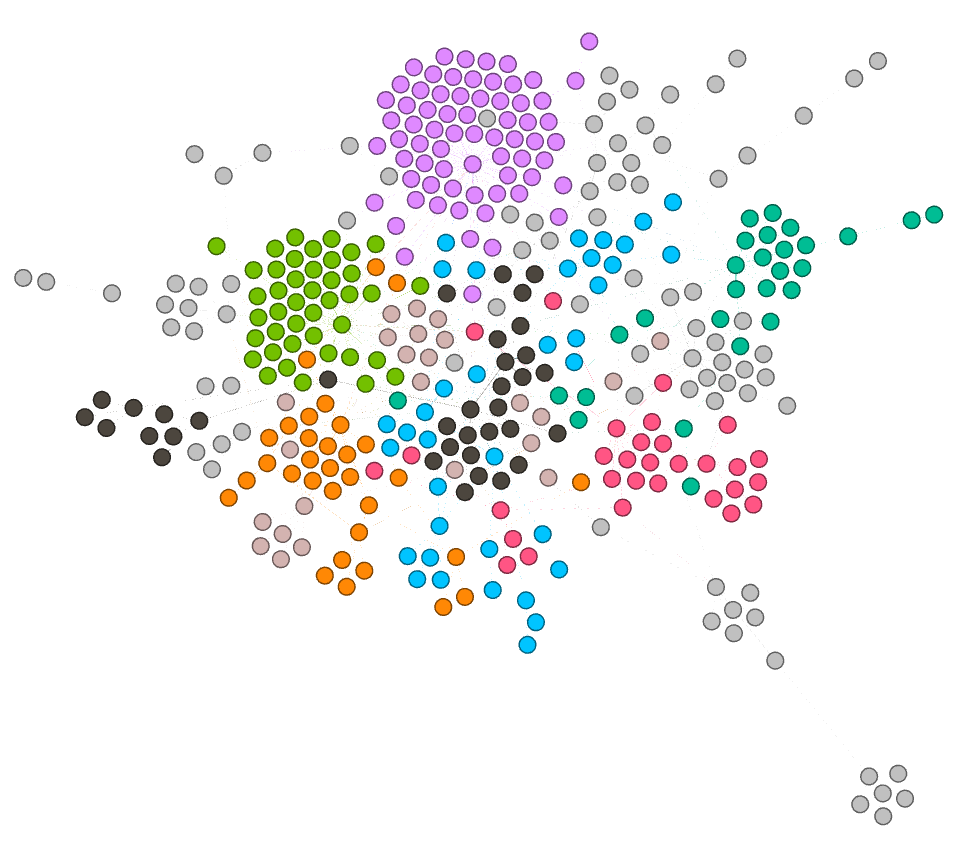
\includegraphics[width=0.80\textwidth]{fig/intro/disjoint_communities.png}
	\caption{Disjoint communities: vertices with unique labels.}
	\label{fig:disjoint_communities}
\end{figure}

Girvan and Newman (2003)\cite{Girvan2003} define a community as a subset of the set of network vertices that are densely connected to each other and have low connection density with the other network vertices not belonging to this subset. This is the definition of community widely accepted and used in the literature. Other nomenclatures analogous to the definition presented by Girvan and Newman are also found as, for example, modules \cite{Lancichinetti2009b}, \textit{clusters} \cite {Lancichinetti2011}, circles \cite{Leskovec2012}, which essentially keep the same concept, but they have specific characteristics that depend on the way the network is modeled and the objective proposed in each research.

%EX:
% modulos - partições do grafo 
% clusters - agrupamento - similaridade
% circulos - cliques de tamanho k

Girvan and Newman (2003)\cite{Girvan2003} further state that a community represents a partition of the original graph, such that each partition maximizes the internal density of the links and minimizes the density of the external links to the obtained parts. This view led to the study and proposition of measures and algorithms that aim to generate optimal partitions. Thus, many works in the literature address the problem of detecting communities as the problem of finding partitions of the network \cite{Dhumal2015, FORTUNATO201075, Lancichinetti2009b, Papadopoulos2012}. The Fig. \ref{fig:disjoint_communities} displays a graph with partitions, identified by vertices with equal colors. Each vertex is associated with only one partition. Each partition can be understood as a community, and the partition set represents a network with disjoint communities.

\begin{figure}[htb]
	\centering
	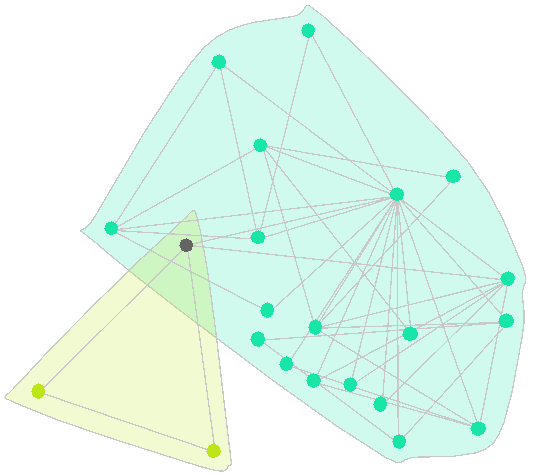
\includegraphics[width=0.80\textwidth]{fig/intro/overlap_communities.png}
	\caption{Overlapping communities: multi-label vertex highlighted.}
	\label{fig:overlap_communities}
\end{figure}

A feature of OSNs that can not be ignored during community detection is the fact that a vertex can be associated with several communities simultaneously \cite{Palla2005}. Communities on these networks do not exactly match different partitions. Social relationships between people often reveal this behavior, with the individual participating in communities defined by family structures, relationships among co-workers, friends of the school, etc. This phenomenon indicates that there are regions of overlap in the graph, with communities being formed by vertices that also belong to other communities. The Fig. \ref{fig:overlap_communities} provides the example of a vertex that is associated with two communities, revealing overlapping communities.

\subsection{Community Detection Algorithms}
\label{sec:comm_algorithms}

Since there are two understandings about how communities can be identified in OSNs, through partitions or overlapping, we will consider in this work the execution of algorithms that return results in both directions. We chose two algorithms that treat communities as partitions of the graph: RAK (initials of the algorithm authors) \cite{Raghavan2007} and INFOMAP (Maps of Information Flow) \cite{Rosvall2008}; and two algorithms that treat communities as overlapping regions in the graph: COPRA (Community Overlap Propagation Algorithm) \cite{Gregory2010} and OSLOM (order Statistics Local Optimization Method) \cite{Lancichinetti2011}. The following is a brief description of the operation of each of them. For more details we recommend reading the comparative analysis made by Fortunato and Lancichinetti \cite{Lancichinetti2009a}, Orman et al. \cite{Orman2012} and Xie et al. \cite{Xie2013}.

\subsubsection*{Disjoint Community Detection}
\label{subsec:disjoint_comm_detection}

The RAK algorithm acts from the Label Propagation concept. It is a simple algorithm that does not require any a priori information about the communities and also does not require the optimization of a predefined objective function, using only information from the network structure. Each vertex is initialized with a unique label and at each iteration of the algorithm the vertex adopts the label that most of its neighbors currently have. If more than one label is used by the same maximum number of neighbours, one of them is chosen randomly. In the end, the communities identified by the vertices that have the same labels. The time complexity of the algorithm is almost linear in the network size, which makes it computationally cheaper.

The algorithm INFOMAP describes random walks along the network encoding the path using two levels of identification, one identifier for the community and another for the vertex within the community, where vertices in different communities can have equal identifiers. The goal is to identify communities in order to minimize the size of the random path description. Intuitively, this is done by clustered together in clusters the vertices that often appear together in random paths. To identify the cluster, INFOMAP uses a greedy algorithm. Initially, each vertex is placed in its own community and communities are merged in order to reduce the expected size of the description of a random walk. Fortunato and Lancichinetti evaluated several algorithms and networks and concluded that INFOMAP was the most reliable of the evaluated methods \cite{Lancichinetti2009a}.


\subsubsection*{Overlap Community Detection}
\label{subsec:overlap_comm_detection}

%%%%%%%%%%%%%%%%%%%%%%%%%%%%%%%%%%%%%%%%%%%%%%%%%%%%%%%%
%%%%%%%%%%%%%%%%%%%%%%%%%%%%%%%%%%%%%%%%%%%%%%%%%%%%%%%%
The COPRA algorithm also uses the label propagation concept and is an extended version of the RAK algorithm for the detection of overlapping communities. A parameter $v$ controls the maximum number of communities a vertex can be associated with. In the tests performed by the authors of the algorithm, the best results for the community evaluation metrics were with the parameter $v$ set at 9, 10 or 11. COPRA also has the advantage of being fast in execution in larger and sparse networks because its complexity of time is essentially linear.

The OSLOM algorithm uses a method capable of differentiating the statistical significance of the real communities with the artificial communities that happen in random networks. Initially the algorithm randomly selects a vertex and adds it to a cluster. Then it analyzes each of the neighbors of this vertex and analyzes if the number of edges in the cluster is above what would be expected in a random network. Thus, at each step, significant vertices are added and insignificant vertices are removed of clusters. The results usually present significant numbers of outliers or singletons (communities formed by only one vertex). The worst case complexity in general is $O(n^2)$, while the exact complexity depends on the community structure of the underlying network under study.

\subsection{Community Quality Measures}
\label{sec:comm_quality}

The task of evaluating communities in OSNs is not trivial. It is not always possible to identify real communities so that some metrics can be used to compare detected communities and ground truth. This problem is known in the literature as ``lack of ground truth'' \cite{Zafarani2015}. The high values of clustering coefficients found in most real graphs indicate that the vertices in these graphs tend to form communities \cite{Girvan7821}, and therefore several metrics are employed from this approach to evaluate the quality of clusters formed and to circumvent the problem of lack of ground truth. In this work we will consider only community quality measures based on the evaluation without ground truth.

There have been a lot of studies about communities in Twitter \cite{McAuley:2012, Lim2012, Amitava:2012, Darmon2015, Amati2015, Mert2016, Achiam2016, Lim2016}, however, the great majority of them aim at discovering communities only in the graph formed by the follow relation. In this work, we also want to investigate the existence and quality of communities that can emerge on the other layers of a Twitter multilayer ego network. To this end, we present in this section some of the most used community quality measures in literature. For this purpose, lets consider a graph $G=(V,E)$, and a set of communities  $\mathcal{C}=\{C_1,\cdots C_{|\mathcal{C}|}\}$ in $G$ found by a given community detection algorithm. A community $C_i$ is a subgraph of $G$. We define $E_{C_i}^{in}$ as set of edges between vertices in $C_i$, $E_{C_i}^{out}$ as the set of edges  from the vertices  in community $C_i$ to the vertices outside $C_i$. Set $V_{C_i}$ is the set of vertices inside community $C_i$.



\subsubsection*{Newman{'}s Modularity}
\label{subsec:newman_modularity}
Newman{'}s modularity \cite{Newman2004b,Newman8577} is a measure of the quality of partitions imposed in a graph by a community detection algorithm.  Modularity measures how different the original graph is from a set of randomized graphs, in terms of the partitions existing in the original graph. For the given community partition of the graph $G$, modularity (Q) is given by \cite{Szymanski2013}:

\begin{equation}\label{eq:newmanModularity}
Q= \sum_{C_i \in \mathcal{C}} \left[ \frac{|E_{C_i}^{in}|}{|E|} - \left(  \frac{\alpha |E_{C_i}^{in}|+|E_{C_i}^{out}|}{\alpha |E|} \right) ^2 \right]
\end{equation}

where $\alpha$ is 1 for directed graphs and 2 for undirected ones. 

For weighted graphs, the definition of modularity is similar to the one corresponding to Eq. \ref{eq:newmanModularity}, however, $|E|$ in the equation is substituted with the sum of the weights of all edges in the graph,  $|E_{C_i}^{in}|$, is substituted with  the sum of the weights of all edges connecting  pairs of vertices inside $C_i$,  and $|E_{C_i}^{out}|$ is replaced by the sum of the weights of all edges connecting a vertex inside $C_i$ to a vertex outside $C_i$.


\subsubsection*{Internal Density}
\label{subsec:internal_density}
Communities usually have a great concentration of links among their internal vertices. Internal density is a local measure which evaluates the number of internal edges inside a community $C_i$ in $\mathcal{C}$ in relation to the total of possible edges inside $C_i$:
\begin{equation}\label{eq:intDensity}
D_{C_i} =\frac{\alpha|E_{C_i}^{in}|}{|V_{C_i}|(|V_{C_i}|-1)}, 
\end{equation} 
where  and $\alpha$ is 1 for directed graphs and 2 for undirected ones. The value of $D_{C_i}$ equals to one if $C_i$ is a clique. A global measure of internal density can be derived for graph $G$, by averaging the internal density values of all communities in $\mathcal{C}$.


\subsubsection*{Modularity-Density}
\label{subsec:modularity_density}
Community detection approaches  that try to maximize Neman{'}s modularity measure has two opposite yet concurrent problems. In
some cases,  a large community is  split into smaller communities. In other cases,  large communities  are formed by merging communities that are smaller than a certain threshold which depends on the total number of edges in the graph and on the degree of inter-connectivity between the communities \cite{Szymanski2013}. The latter problem is known as the resolution limit problem \cite{Fortunato36}. 

To solve both of the above mentioned problems, Chen, Nguyen and Szymanski \cite{Szymanski2013} proposed a measure termed  Modularity Density, as an alternative to modularity. 
Their measure modifies Newman{'}s modularity by introducing  two modifications in the original modularity formula: {\em Split Penalty} and {\em density}. Split penalty is the fraction of edges that connect vertices of different communities and solves the problem of favoring small communities. Density solves the resolution problem and is composed of two measures: internal density of each community (see Section \ref{subsec:internal_density}) and an the concept of internal density extended to consider a pair of communities. The Modularity-Density measure is defined as:

\begin{equation}\label{eq:modDensity}
\begin{array}{lll}
Q_{d} (G) =   \sideset{}{}\sum\limits_{C_i \in \mathcal{C}} \left[\frac{|E_{c_i}^{in}|}{|E|}D_{C_i} -    \left( \frac{\alpha |E_{C_i}^{in}| + |E_{C_i}^{out}|}{\alpha |E|}D_{C_i}\right)^2 
 - \sum\limits_{\substack{C_j \in \mathcal{C}\\C_j\neq C_i}} \frac{|E_{C_i,C_j}|}{\alpha|E|}D_{C_i,C_j}\right],\\
%&d_{C_i}= \frac{\alpha|E_{C_i}^{in}|}{V_{C_i}(|V_{C_i}|-1)}&,\\
%&d_{C_i,C_j} = \frac{|E_{C_i,C_j}|}{|V_{C_i}| |V_{C_j}|}&
\end{array}             
\end{equation} \vspace{4mm}
where $D_{C_i}$ is the internal density of community $C_i$ as defined in Eq. \ref{eq:intDensity}, and $D_{C_i,C_j}$ is  the pair-wise density between community $C_i$ and $C_j$ and is defined as:
$$ d_{C_i,C_j} = \frac{|E_{C_i,C_j}|}{|V_{C_i}| |V_{C_j}|}, $$
where $E_{C_i,C_j}$ is the set of edges from community $C_i$ to
community $C_j$. 


\subsubsection*{Conductance}
\label{subsec:conductance}
Conductance  measures the fraction of the
total number of edges that point outside the community:  
\begin{equation}
\label{eq:conductance}
\phi (C) =\frac{|E_{C_i}^{out}|}{2|E_{C_i}^{in}| +|E_{C_i}^{out}|}.
\end{equation}

As occurs with density, a global value of conductance can be obtained by averaging the conductance values over all communities. A smaller value of average conductance means better community quality. But the greatest the average conductance the more interconnected are the communities. 